%%%%%%%%%%%%%%%%%%%%%%%%%%%%%%%%%%%%%%%%%
% Short Sectioned Assignment
% LaTeX Template
% Version 1.0 (5/5/12)
%
% This template has been downloaded from:
% http://www.LaTeXTemplates.com
%
% Original author:
% Frits Wenneker (http://www.howtotex.com)
%
% License:
% CC BY-NC-SA 3.0 (http://creativecommons.org/licenses/by-nc-sa/3.0/)
%
%%%%%%%%%%%%%%%%%%%%%%%%%%%%%%%%%%%%%%%%%

%----------------------------------------------------------------------------------------
%	PACKAGES AND OTHER DOCUMENT CONFIGURATIONS
%----------------------------------------------------------------------------------------

\documentclass[paper=a4, fontsize=11pt]{scrartcl} % A4 paper and 11pt font size

\usepackage[T1]{fontenc} % Use 8-bit encoding that has 256 glyphs
%\usepackage{fourier} % Use the Adobe Utopia font for the document - comment this line to return to the LaTeX default
\usepackage[english]{babel} % English language/hyphenation
\usepackage{amsmath,amsfonts,amsthm} % Math packages
%\usepackage[version=3]{mhchem} % Package for chemical equation typesetting
\usepackage{siunitx} % Provides the \SI{}{} and \si{} command for typesetting SI units
\usepackage{graphicx} % Required for the inclusion of images
%\usepackage{natbib} % Required to change bibliography style to APA
\usepackage{authblk}
\usepackage{indentfirst}
\usepackage{subcaption}
\usepackage{wrapfig}
\usepackage{multirow}
\usepackage{hyperref}
\usepackage{float}
\usepackage{url}
\usepackage{booktabs}
\usepackage{times}

\usepackage{lipsum} % Used for inserting dummy 'Lorem ipsum' text into the template

\usepackage{sectsty} % Allows customizing section commands
\allsectionsfont{\centering \normalfont\scshape} % Make all sections centered, the default font and small caps

\usepackage{geometry}
\geometry{left=2.5cm,right=2.5cm,top=2.5cm,bottom=2.5cm}

\graphicspath{{images/}{figures/}}

\usepackage{fancyhdr} % Custom headers and footers
\pagestyle{fancyplain} % Makes all pages in the document conform to the custom headers and footers
\fancyhead{} % No page header - if you want one, create it in the same way as the footers below
\fancyfoot[L]{} % Empty left footer
\fancyfoot[C]{} % Empty center footer
\fancyfoot[R]{\thepage} % Page numbering for right footer
\renewcommand{\headrulewidth}{0pt} % Remove header underlines
\renewcommand{\footrulewidth}{0pt} % Remove footer underlines
\setlength{\headheight}{13.6pt} % Customize the height of the header

\numberwithin{equation}{section} % Number equations within sections (i.e. 1.1, 1.2, 2.1, 2.2 instead of 1, 2, 3, 4)
\numberwithin{figure}{section} % Number figures within sections (i.e. 1.1, 1.2, 2.1, 2.2 instead of 1, 2, 3, 4)
\numberwithin{table}{section} % Number tables within sections (i.e. 1.1, 1.2, 2.1, 2.2 instead of 1, 2, 3, 4)

\linespread{1.213}
%\setlength{\parskip}{0.5\baselineskip}

%\setlength\parindent{0pt} % Removes all indentation from paragraphs - comment this line for an assignment with lots of text

%----------------------------------------------------------------------------------------
%	TITLE SECTION
%----------------------------------------------------------------------------------------

\newcommand{\horrule}[1]{\rule{\linewidth}{#1}} % Create horizontal rule command with 1 argument of height

\title{	
	\normalfont \normalsize 
	\textsc{Philipps-Universitaet Marburg, The Department of Physics} \\ [25pt] % Your university, school and/or department name(s)
	\horrule{0.5pt} \\[0.4cm] % Thin top horizontal rule
	\huge Computational Physics II: Assignment 1 \\ % The assignment title
	\horrule{2pt} \\[0.5cm] % Thick bottom horizontal rule
}

\author{Houchen \textsc{Li}} % Your name

\date{\normalsize\today} % Today's date or a custom date

\begin{document}

\maketitle % Print the title

%----------------------------------------------------------------------------------------
%	PROBLEM 1
%----------------------------------------------------------------------------------------

\section{Dice}

The key point of this task is to find a proper way plotting the histograms. Since the duplets and the triplets are multi-dimensional random vectors, plot the probabilities of each sample versus a multi-dimensional phase space may not be such evident. My approach is to use a senary scale to transfer the digits to natural integers, for example, I allocate duplets and triplets as \\
\begin{minipage}[b]{0.4\linewidth}
\centering
\begin{gather*}
	\left( 11 \right)_6\sim \left(0\right)_{10}\\
	\left( 12 \right)_6\sim \left(1\right)_{10}\\
	\vdots\\
	\left( ij \right)_6\sim \left( \left(i-1\right)\times 6+\left(j-1\right) \right)_{10}\\
	\vdots\\
	\left( 66 \right)_6\sim \left(35\right)_{10}
\end{gather*}
\end{minipage}
\begin{minipage}[b]{0.59\linewidth}
\centering
\begin{gather*}
	\left( 111 \right)_6\sim \left(0\right)_{10}\\
	\left( 112 \right)_6\sim \left(1\right)_{10}\\
	\vdots\\
	\left( ijk \right)_6\sim \left( \left(i-1\right)\times 6^2+\left(j-1\right)\times 6+\left(k-1\right) \right)_{10}\\
	\vdots\\
	\left( 666 \right)_6\sim \left(215\right)_{10}
\end{gather*}
\end{minipage} \\
Thus, each sample can be represent by a given integer. Then I use this integer as the x-axis while the probability as the y-axis to do plotting, the histograms of dulplets and triplets are presented in Figure~\ref{fig:dice_1}. \par
\begin{figure}[!ht]
	\centering
	\begin{subfigure}[b]{0.495\textwidth}
		\centering
		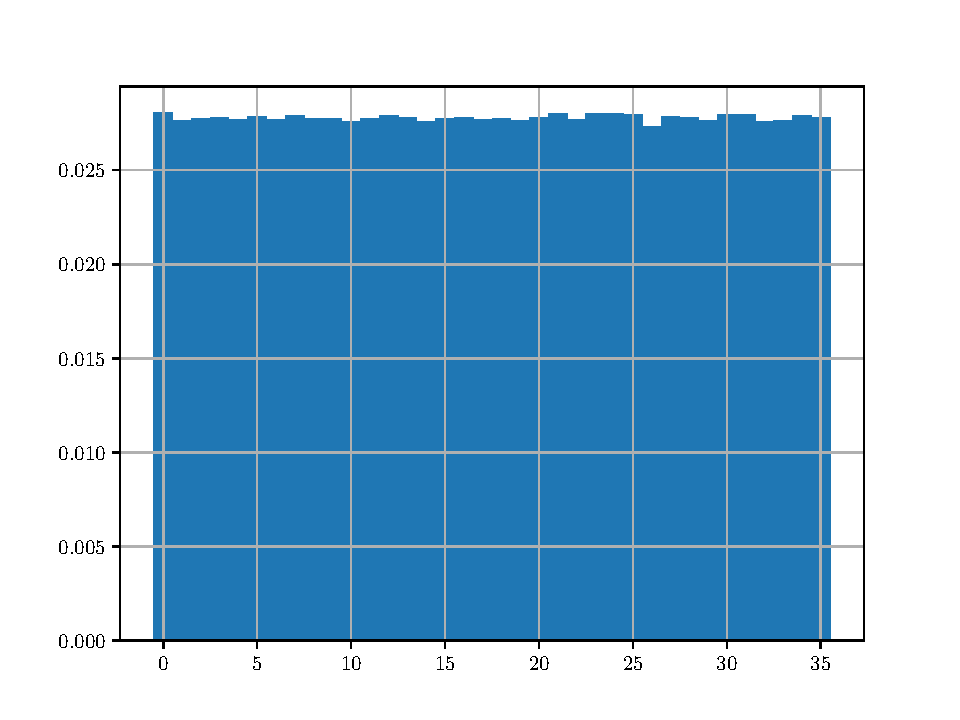
\includegraphics[width=\linewidth]{figure_1_a.pdf}
		\caption{}
		\label{fig:dice_1:a}
	\end{subfigure}
	\begin{subfigure}[b]{0.495\textwidth}
		\centering
		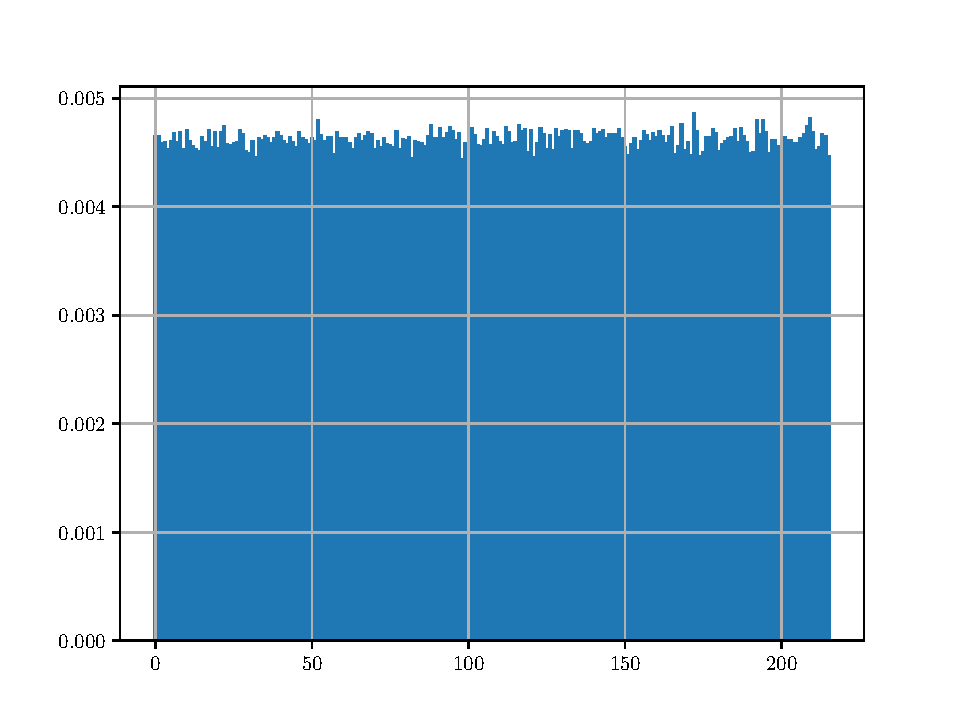
\includegraphics[width=\linewidth]{figure_1_b.pdf}
		\caption{}
		\label{fig:dice_1:b}
	\end{subfigure}
	\caption{The histograms for the duplets and triplets of dice rolling arrays with a size of \num{1e6}: (\ref{fig:dice_1:a}) the distribution of the duplets; (\ref{fig:dice_1:b}) the distribution of the triplets.}
	\label{fig:dice_1}
\end{figure}
The distribution of duplets seem to be a uniform distribution, which evident the pair correlation of the random number generator is nearly ignorable. However, the distribution of the triplets provides some strange information. There should be 216 bars in the histogram instead of 36 bars, since our sample space has a size of 216 rather than 36. I think the some of the samples are not covered by the random triplets due to the collapse of the zero correlation, resulting in such a phenomenon. In the end, a conclusion, the random number generator can work without the pair correlation but still may crash if being involved with triplets correlation, can be extracted. \par

%----------------------------------------------------------------------------------------
%	PROBLEM 2
%----------------------------------------------------------------------------------------

\section{M{\"a}xchen or Mia}

The comparing relation is going as:
\begin{gather*}
	\text{rank}(31) < \text{rank}(32) < \text{rank}(41) < \text{rank}(42) < \text{rank}(43) < \text{rank}(51) < \text{rank}(52) < \text{rank}(53) < \\\text{rank}(54) < \text{rank}(61) < \text{rank}(62) < \text{rank}(63) < \text{rank}(64) < \text{rank}(65) < \text{rank}(11) < \text{rank}(22) < \\\text{rank}(33) < \text{rank}(44) < \text{rank}(55) < \text{rank}(66) < \text{rank}(21).
\end{gather*}
By using python, I generated about \num{1d6} such duplet groups. Then use the comparing relation to check the duration of non-decreasing series. The distribution of the non-decreasing series is presented in Figure~\ref{fig:maexchen_1}. \par
\begin{figure}[!ht]
	\centering
	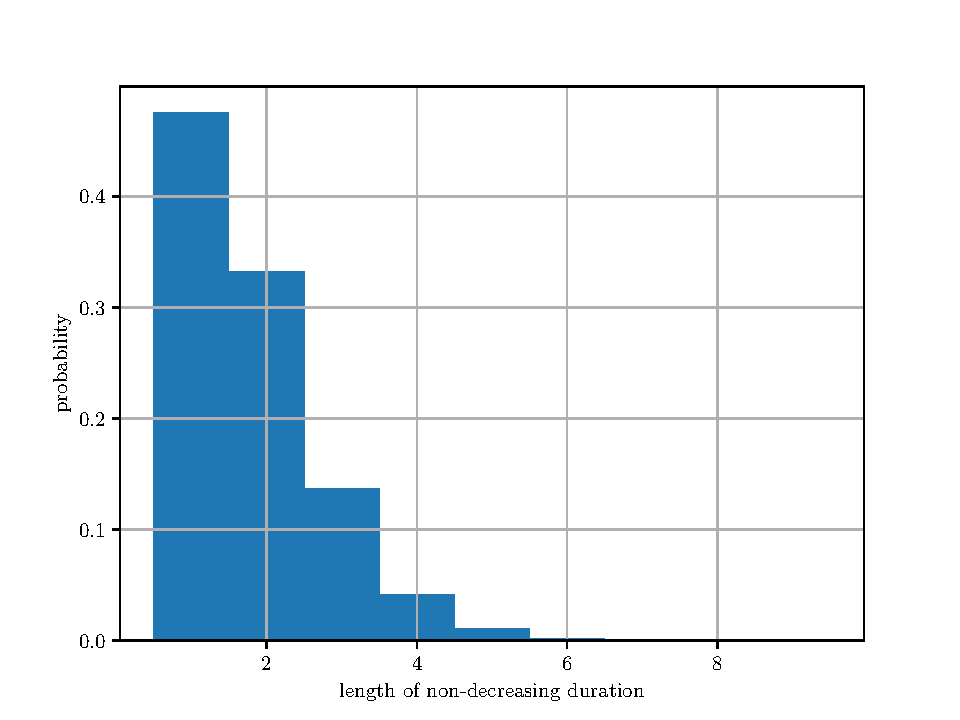
\includegraphics[width=0.495\linewidth]{figure_2.pdf}
	\caption{The distribution of the non-decreasing duration.}
	\label{fig:maexchen_1}
\end{figure}

%----------------------------------------------------------------------------------------
%	PROBLEM 3
%----------------------------------------------------------------------------------------

\section{Non-uniform random variables}

The transformation from a uniform distribution to a power distribution both at interval \(\left( 0,1 \right)\) goes as below:
\begin{align*}
	Ax^\alpha\mathrm{d}x&=\mathrm{d}\xi\\
	A\left( \alpha+1 \right)^{-1}\mathrm{d}x^{\alpha+1}&=\mathrm{d}\xi\\
	x&=\left[A^{-1} \left( \alpha+1 \right)\xi\right]^{\frac{1}{\alpha+1}}\\
	x&=\xi^{\frac{1}{\alpha+1}}
\end{align*}
where \(A\) is a normalization factor. The restriction for \(\alpha\) is that the integral of the power distribution shall exist for \(\left( 0,1 \right)\). Only when \(\alpha>-1\), can this integral exist. \par
Figure~\ref{fig:non-uniform_1} gives the histograms of power distribution with different \(\alpha\).
\begin{figure}[!ht]
	\centering
	\begin{subfigure}[b]{0.495\textwidth}
		\centering
		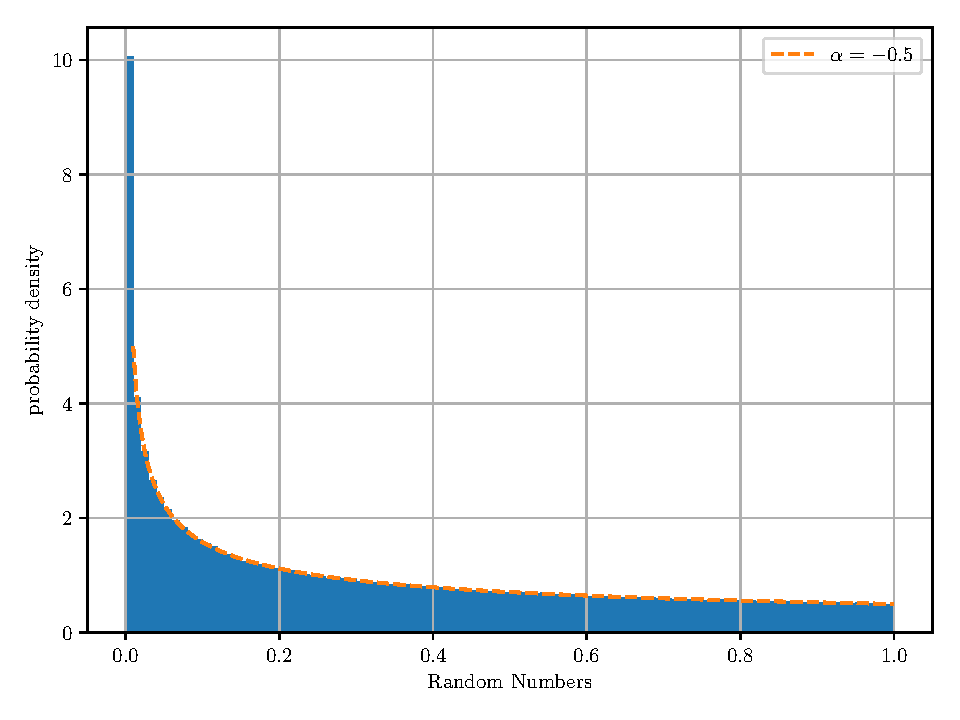
\includegraphics[width=\linewidth]{figure_3_a.pdf}
		\label{fig:non-uniform_1:a}
	\end{subfigure}
	\begin{subfigure}[b]{0.495\textwidth}
		\centering
		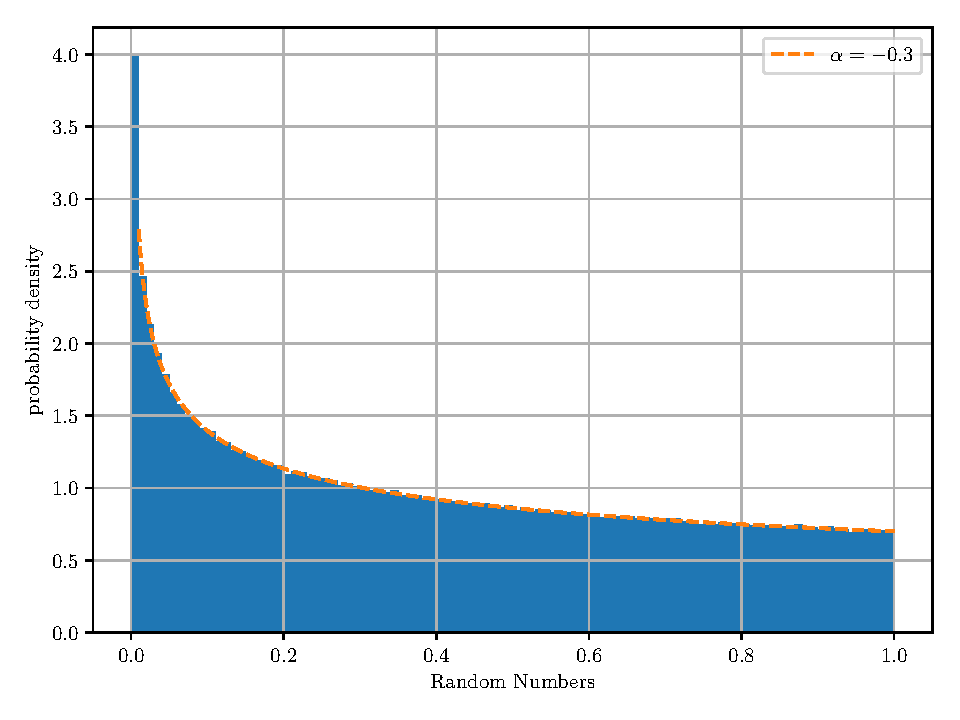
\includegraphics[width=\linewidth]{figure_3_b.pdf}
		\label{fig:non-uniform_1:b}
	\end{subfigure}
	\begin{subfigure}[b]{0.495\textwidth}
		\centering
		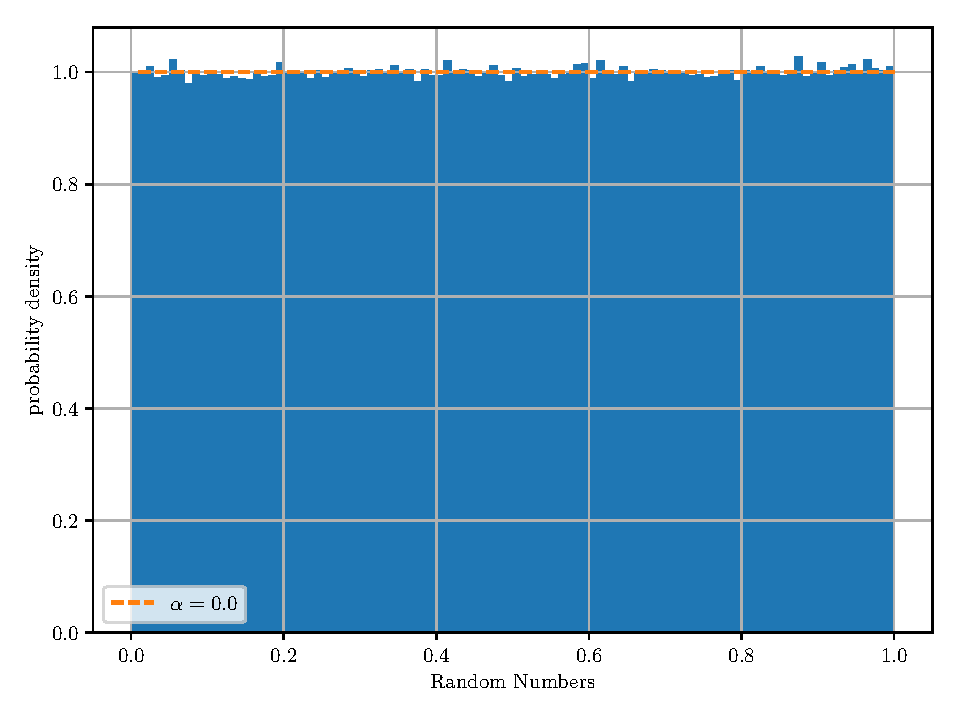
\includegraphics[width=\linewidth]{figure_3_c.pdf}
		\label{fig:non-uniform_1:c}
	\end{subfigure}
	\begin{subfigure}[b]{0.495\textwidth}
		\centering
		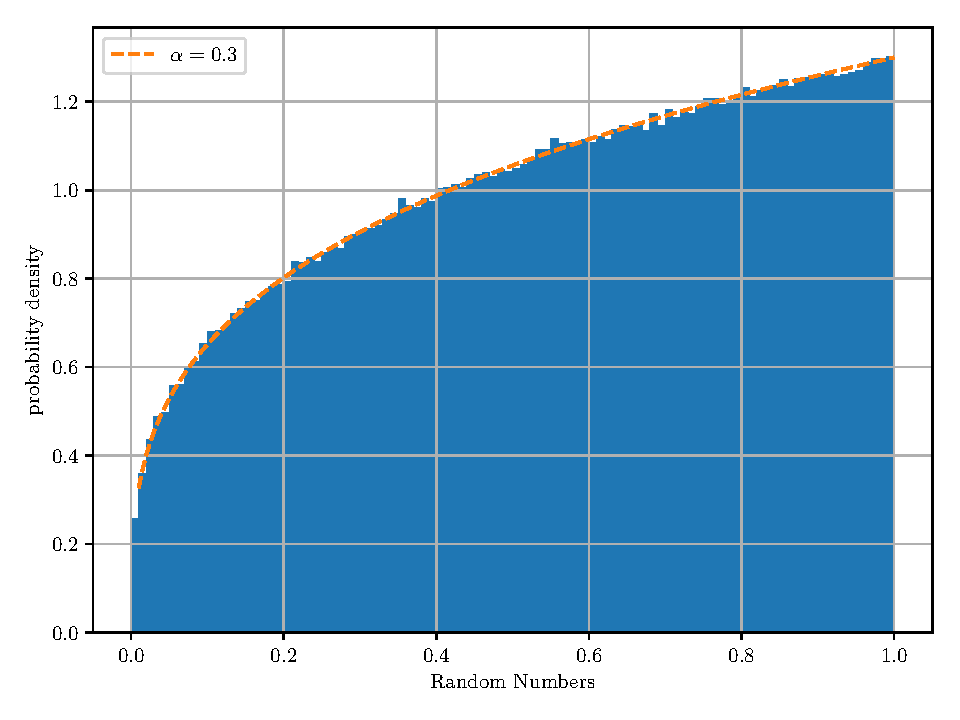
\includegraphics[width=\linewidth]{figure_3_d.pdf}
		\label{fig:non-uniform_1:d}
	\end{subfigure}
	\begin{subfigure}[b]{0.495\textwidth}
		\centering
		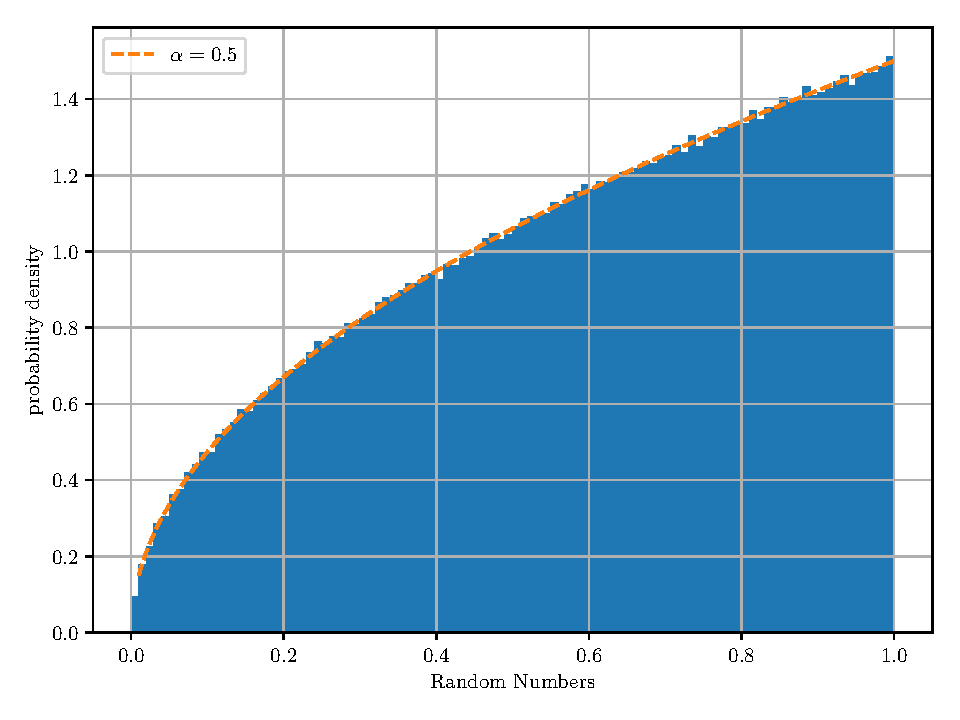
\includegraphics[width=\linewidth]{figure_3_e.pdf}
		\label{fig:non-uniform_1:e}
	\end{subfigure}
	\begin{subfigure}[b]{0.495\textwidth}
		\centering
		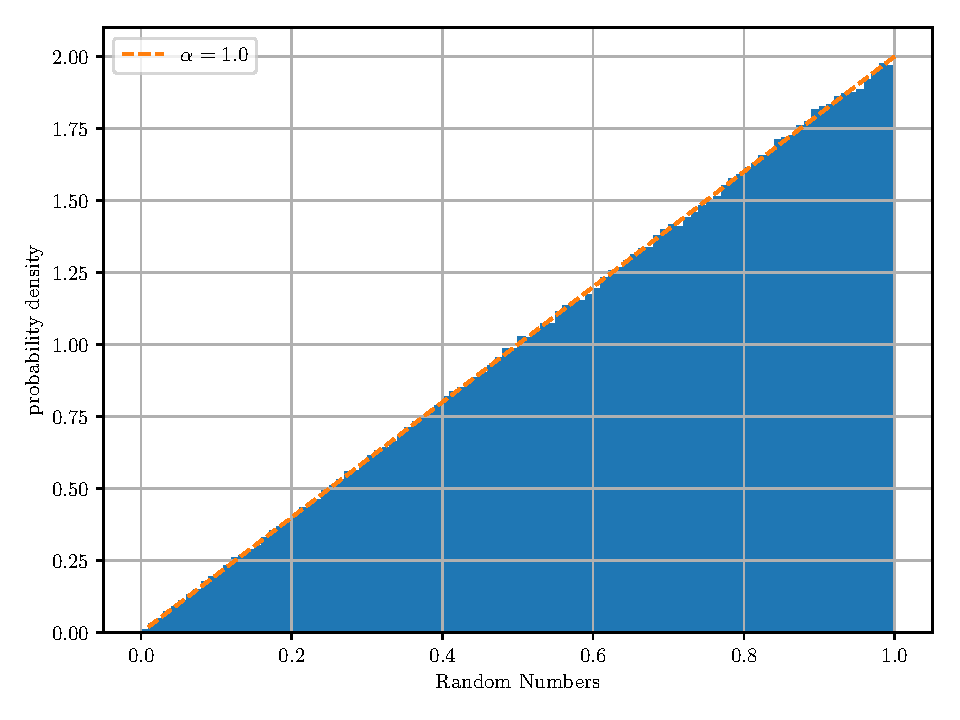
\includegraphics[width=\linewidth]{figure_3_f.pdf}
		\label{fig:non-uniform_1:f}
	\end{subfigure}
	\begin{subfigure}[b]{0.495\textwidth}
		\centering
		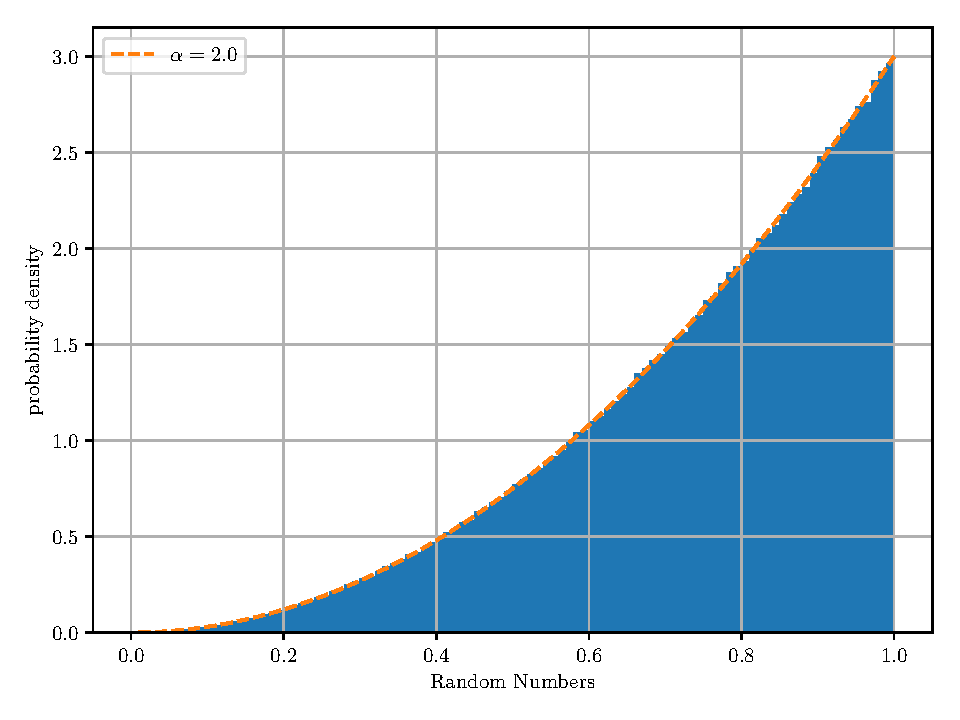
\includegraphics[width=\linewidth]{figure_3_g.pdf}
		\label{fig:non-uniform_1:g}
	\end{subfigure}
	\begin{subfigure}[b]{0.495\textwidth}
		\centering
		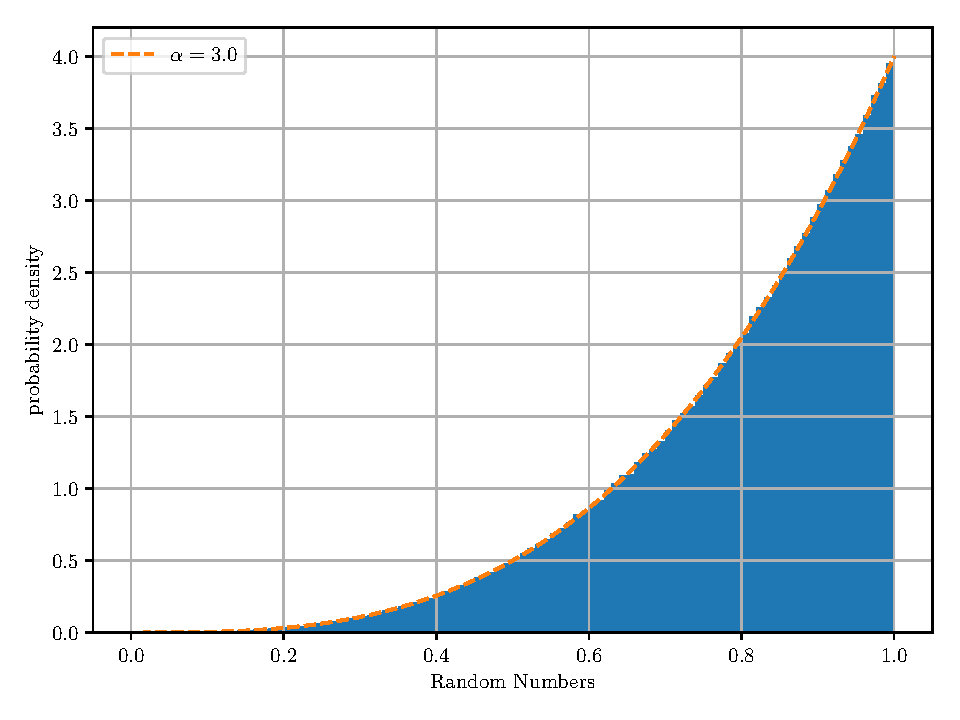
\includegraphics[width=\linewidth]{figure_3_h.pdf}
		\label{fig:non-uniform_1:h}
	\end{subfigure}
	\caption{the power random distribution transformed from uniform distribution with different \(\alpha\).}
	\label{fig:non-uniform_1}
\end{figure}\par

%----------------------------------------------------------------------------------------

\end{document}
